\documentclass[conference]{IEEEtran}
\usepackage{times}
\usepackage{graphicx}
\usepackage{booktabs}
\usepackage{latexsym,amssymb,amsmath} % for \Box, \mathbb, split, etc.
%\usepackage{path}
\usepackage{url}
\usepackage{verbatim}
\usepackage[numbers]{natbib}
\usepackage{amsfonts}
\usepackage{color}

\newcommand{\stnote}[1]{\textcolor{blue}{\textbf{ST: #1}}}
\newcommand{\jgonote}[1]{\textcolor{green}{\textbf{JGO: #1}}}

\usepackage{algorithmic}

\newcommand{\mytitle}[0]{Autonomously Acquiring Models of Objects for
  Instance-Based Grasping}

\pdfinfo{
   /Author ()
   /Title  (\mytitle)
   /CreationDate (D:20101201120000)
   /Subject (Robots)
   /Keywords ()
}



\makeatletter
\setlength{\arraycolsep}{2\p@} % make spaces around "=" in eqnarray smaller
\makeatother


% begin of personal macros
\newcommand{\half}{{\textstyle \frac{1}{2}}}
\newcommand{\eps}{\varepsilon}
\newcommand{\myth}{\vartheta}
\newcommand{\myphi}{\varphi}

\newcommand{\IN}{\mathbb{N}}
\newcommand{\IZ}{\mathbb{Z}}
\newcommand{\IQ}{\mathbb{Q}}
\newcommand{\IR}{\mathbb{R}}
\newcommand{\IC}{\mathbb{C}}
\newcommand{\Real}[1]{\mathrm{Re}\left({#1}\right)}
\newcommand{\Imag}[1]{\mathrm{Im}\left({#1}\right)}

\newcommand{\norm}[2]{\|{#1}\|_{{}_{#2}}}
\newcommand{\abs}[1]{\left|{#1}\right|}
\newcommand{\ip}[2]{\left\langle {#1}, {#2} \right\rangle}
\newcommand{\der}[2]{\frac{\partial {#1}}{\partial {#2}}}
\newcommand{\dder}[2]{\frac{\partial^2 {#1}}{\partial {#2}^2}}

\newcommand{\nn}{\mathbf{n}}
\newcommand{\xx}{\mathbf{x}}
\newcommand{\uu}{\mathbf{u}}

\newcommand{\junk}[1]{{}}

% set two lengths for the includegraphics commands used to import the plots:
\newlength{\fwtwo} \setlength{\fwtwo}{0.45\textwidth}


\renewcommand{\labelitemi}{}
\renewcommand{\labelitemii}{}
\renewcommand{\labelitemiii}{}


% end of personal macros
% \input{inputFile.tex}


\begin{document}
%\DeclareGraphicsExtensions{.jpg}


\title{\mytitle{}}

\author{Author Names Omitted for Anonymous Review. Paper-ID [add your ID here]}

\maketitle


\begin{abstract}
Manipulating objects is an important task for robots that help people
in the home, in factories, and in hospitals.  General-purpose
pick-and-place requires object recognition, pose estimation, and grasp
planning; existing solutions cannot reliably recognize or pick up an
object the robot has never encountered before~\citep{}.  However in
many applications, general-purpose pick-and-place is not required: the
robot would be useful if it could recognize and manipulate the small
set of objects most important in that application, but do so with high
reliability.  To address this problem, we define a SLAM-based approach
which enables the robot to actively acquire visual and grasp models of
novel objects by moving its sensor and trying grasps, integrating
information over time.  Unlike conventional SLAM, in our model the
hidden state is the object pose, and the map consists of invariant
features of the object such as appearance information and grasp
points.  Our approach converts the task of {\em category recognition}
(pick up any mug) to {\em instance recognition} (pick up this mug),
enabling models to be autonomously acquired for specific objects.
Using our approach, a robot can interact with an object for ten
minutes, and then reliably localize (90\%) and manipulate it (90\%
successful grasps).


%% Robots need to pick stuff up.
%% %
%% Perception can structure data, structured data facilitates planning, planning allows more principled perception.
%% %
%% The tasks of robotic perception, planning, and control will all benefit from
%% a design paradigm which allows them to be jointly programmed.
%% %
%% So we contribute an implementation \emph{NODE} which facilitates the design and 
%% execution of versatile and scalable MDPs structured in what we call a
%% Von Neumann MDP pattern. 
%% %
%% We form a closed loop through perception and planning, allowing them to interact by means of structured data.
%% %
%% Our system incorporates online, human-in-the-loop algorithms. Non-technical human participants can easily
%% teach and collaborate with the system.
\end{abstract}


% First paragraph: What is the problem we are trying to solve? I
% think it's something about enabling a robot to robustly perceive and
% manipulate native objects, so that it can carry out tasks such as
% assisting at childcare, cooking, or in hospitals.
% Second paragraph: Why hasn't previous work addressed this problem?
% I think it's something about the focus on category recognition, not
% doing pose estimation, and training methods that require an expert
% user and an annotated corpus.
% Third paragraph: What do we propose to do to address this problem?
% Fourth paragraph: Our high-level technical approach
% Fifth paragraph: How do we know it works? Why is it cool?
% Something about an evaluation and something about a robotic
% demonstration.

\section{Introduction}
Robotic assistants will assist us at childcare, help us cook, and provide service to
doctors, nurses, and patients in hospitals. Many such tasks require a robot to
robustly perceive and manipulate objects. 
Conventional systems are capable of perception and manipulation in a limited sense.
Some systems require training by a human operator on an object to object basis, which 
is time consuming and can be difficult for a non-expert to perform ~\citep{ork14, lai11, lai11a}. There 
do exist some systems which
do not require training on a per object basis, but they are computationally expensive and do not enjoy the
highest accuracy or precision and have not been demonstrated for grasping~\citep{guadarrama14}.

To obtain the benefits of both approaches, we propose a system which trains itself 
to recognize and manipulate the specific objects it will need to use during future
collaborations with humans. 
Our system is powerful because it learns to identify and grasp on 
a per object basis. Our system is portable, convenient, and general because the expert knowledge it employs
is built into the algorithms which it uses to train itself, requiring only basic
interaction from a non-technical human collaborator.

Our contribution is an algorithm which allows a robot to autonomously
train its subsystems, together with three applications of the
algorithm to the tasks mentioned above.  The first application is
recognizing the category of an object and the second application is
estimating the pose of the object, both of which we accomplish with
simple and robust computer vision algorithms combined with our
  proposed algorithm for autonomous collection of training data. The
third application is grasping the object, which we accomplish with
visual servoing techniques. Each of these components is well
understood in its own right, and existing methods allow expert users
to train systems to accomplish these tasks satisfactorily.

When we apply the algorithm to the recognition task, the robot trains
the recognition system to discriminate between object instance
categories. When we apply the algorithm to the pose estimation task,
the robot trains the pose estimation system to determine which pose an
identified object holds.  When we apply the algorithm to the grasping
task, the robot trains the grasping system to successfully and quickly
pick and place the target object.  Crucially, our algorithm can
recognize when it is doing a poor job at learning and asks a human
collaborator to manually annotate information in those cases.



It works because our experiments tell us so. This is how well they
work: .  Thus we see an improvement over expert trained systems (cite
usability results), and is an improvement over un-annotated systems
(cite success rates, the ability to generalize, and the low
computational overhead since we don't crunch expensive features or do
heavy classification at run time).

\stnote{We have to say the right things about ORK.  Why does ORK suck?
  Why doesn't it already solve the problem?}


\section{Object Detection and Pose Estimation}

We first describe our instance-based object detection and pose
estimation pipeline, which uses standard computer vision algorithms
combined to achieve a simple software architecture, a high frame rate,
and high accuracy at recognition and pose estimation.  This pipeline
can be manually trained by an expert to reliably detect and grasp
objects.  Additionally, section~\ref{sec:training} describes our
approach to enabling a robot to autonomously train this pipeline by
actively collecting images and training data from the environment.

\subsection{Object Recognition}
\jgonote{Cover BING, SIFT, BoW, typical training pipelines, and RGB-D
  approaches popular in the robotics community.} 

Our recognition pipeline takes RGB-D video from the robot, proposes a
small number of candidate object bounding boxes in each frame, and
classifies each candidate bounding box as belonging to a previously
encountered object class. Our object classes consist of object
instances rather than pure object categories.  Using instance
recognition means we cannot reliably detect categories, such as
``mugs,'' but the system will be able to detect, localize, and grasp
the specific instances for which it has models with much higher speed
and accuracy.

To generate candidate bounding boxes, we first apply the BING
objectness detector~\citep{cheng14} to the image, which returns a set
$\{B_i\}$ of thousands of approximate object bounding boxes in the
image. This process substantially reduces the number of bounding boxes
we need to consider but is still too large for us to process in real
time. Besides, even good bounding boxes from BING are typically not
aligned to the degree that we require. Therefore, we use integral
images to efficiently compute the per-pixel map:
\begin{align}
J(p) = \sum_{B \in \{B_i\} s.t. p \in B} \frac{1}{Area(B)}.
\end{align}
We then apply the Canny edge detector with hysteresis ~\citep{} to find the connected components of bright
regions in the map $J(p)$, which correspond with high probability to objects in the image. We form
our candidate object bounding boxes by taking the smallest bounding box which surrounds each connected component.
These bounding boxes make it easy to gather training data and to perform inference in real time, but at
the expense of poorly handing occulusion as overlapping objects are fused into the same bounding box.
It is possible to search within the proposed bounding boxes to better handle occlusion.

For each object $c$ we wish to classify, we gather a set of example crops $E_c$ which are candidate
bounding boxes (derived as above) which contain $c$. We extract dense SIFT features ~\citep{} from all boxes of
all classes and use k-means to extract a visual vocabulary of SIFT features ~\citep{}. We then construct a
BoW feature vector for each image and augment it with a histogram of colors which appear in that image.
The augmented feature vector is incorporated into a k-nearest-neighbors model which we use to classify
objects at inference ~\citep{}.

The use of SIFT features is motivated by the instance level nature of our task. State-of-the-art vision
methods typically use HOG ~\citep{} or CNN ~\citep{} features, but that choice is motivated by category
level recognition. \stnote{What about category level recognition motivates HOG or CNN?  Can you be more specific?}

We use kNN because it is easy to rebuild online, which is a key property a classifier should enjoy
if it is to interact with our framework in real time. State-of-the-art computer vision classifiers
currently employ SVM's ~\citep{} or other models which require expensive training. Using such a model would
introduce a training step in the inside loop of our data collection process, which would be costly
in either engineering or time.  It is possible to use kNN during the online collection process and then
train a stronger classifier in the background at higher latency, essentially introducing a cascading step
in the data collection process.

\begin{figure*}
  \begin{center}
    \begin{tabular}{l c r}
      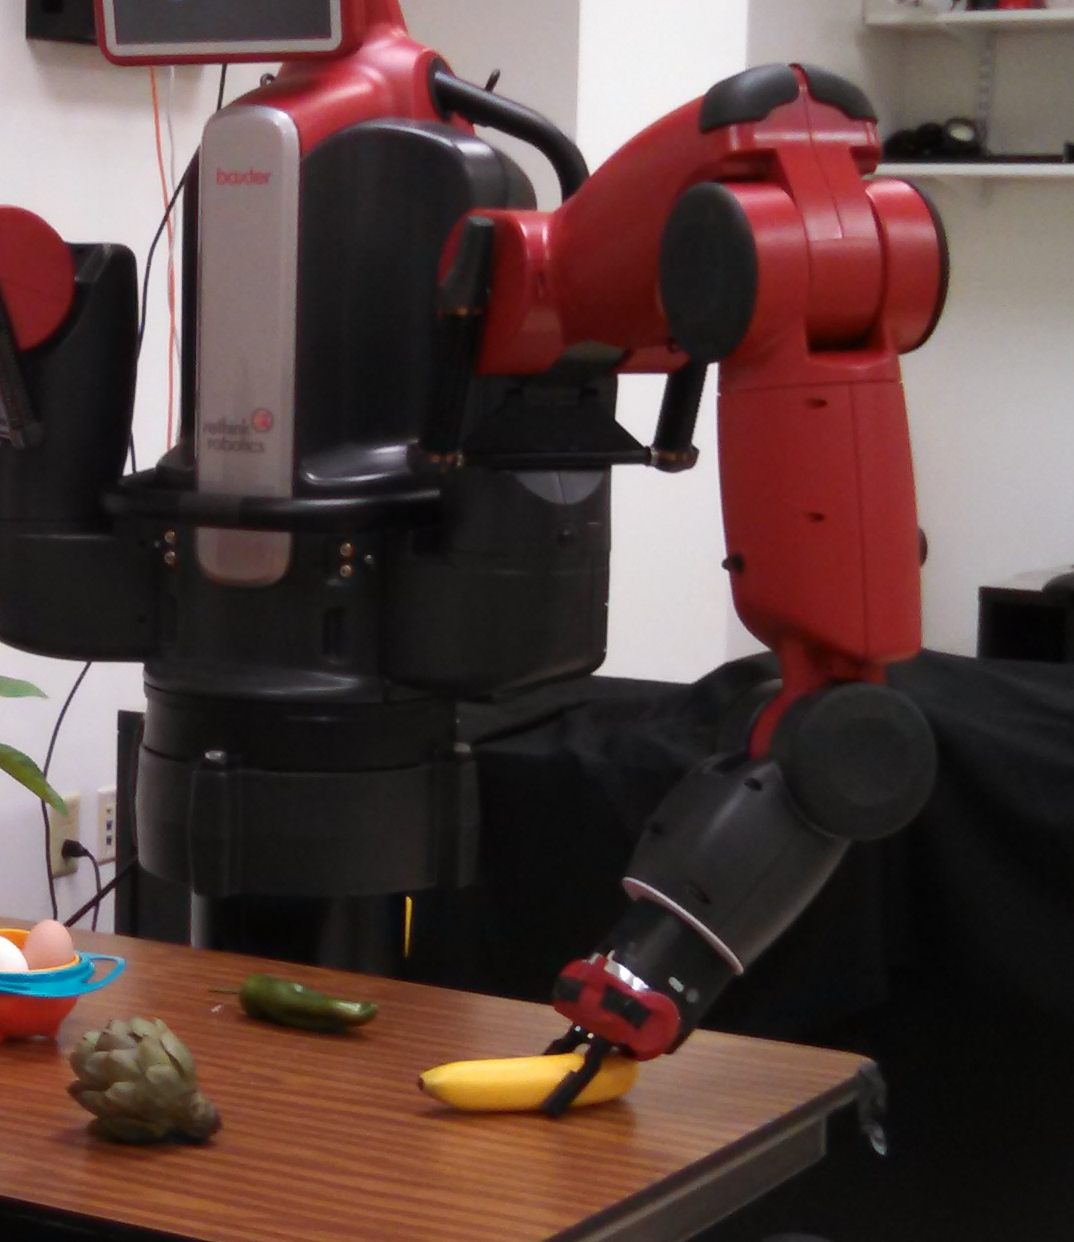
\includegraphics[width=160px, height=120px]{kinect.png} &
      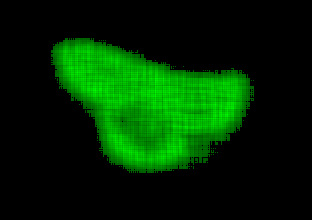
\includegraphics[width=160px, height=120px]{objectness.png} &
      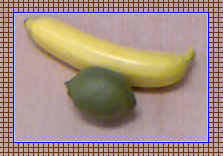
\includegraphics[width=160px, height=120px]{blueBoxes.png} \\
    \end{tabular}
  \end{center}
  \caption{The Object Detection Pipeline. Left: The raw image as viewed through the kinect. 
    Center: The computed objectness map J. Right: Labeled object detections. \stnote{Use subfigure}}
\end{figure*}

 
\subsection{Pose Estimation}
\jgonote{Computer vision approaches, geometry and point cloud based approaches. Dieter Fox's automatic
training pipeline (how well developed is it? we may need to sell our approach as being a 
general algorithm for allowing a robot to train arbitrary subsystems in order to differentiate 
ourselves.)}
We tackle the pose estimation problem using the same classification pipeline that we use for
object recognition. We train a separate pose classifier for each object class. This time, the class
assigned to each training example is the orientation from which the object is viewed in that example.
During inference, we first determine the object class of a candidate bounding box, and once the class
is known we apply the corresponding pose classifier to determine the orientation from which we
are viewing the object. We combine this orientation with position information from the point cloud
information derived from the D channel of the RGB-D video to form a full pose estimate.

\subsection{Object Grasping}
\jgonote{Including open and closed loop paradigms, learning specific and generic grasp models.}

We consider a setting where a robotic arm
with 7 degrees of freedom grasps objects with a parallel plate gripper which adds
an additional degree of freedom, but much of what we discuss could be extended to other
arms and grippers, for instance the universal jamming gripper ~\citep{}.

We use a dual rate PID controller in the sense that we use two sets of PID coefficients. The
first set is for making large adjustments when the aim if off by a significant amount. The
second set is for making small adjustments when aim is close to the target.

Our system is distributed and thus at times there is an appreciable amount of latency between
communicating components. Care is taken to synchronize robot movement with object detection
reports, allowing only a fixed amount of movement per report.

Visual servoing tutorial paper: \citep{chaumette06}

\begin{figure*}
  \begin{center}
    \begin{tabular}{l c}
      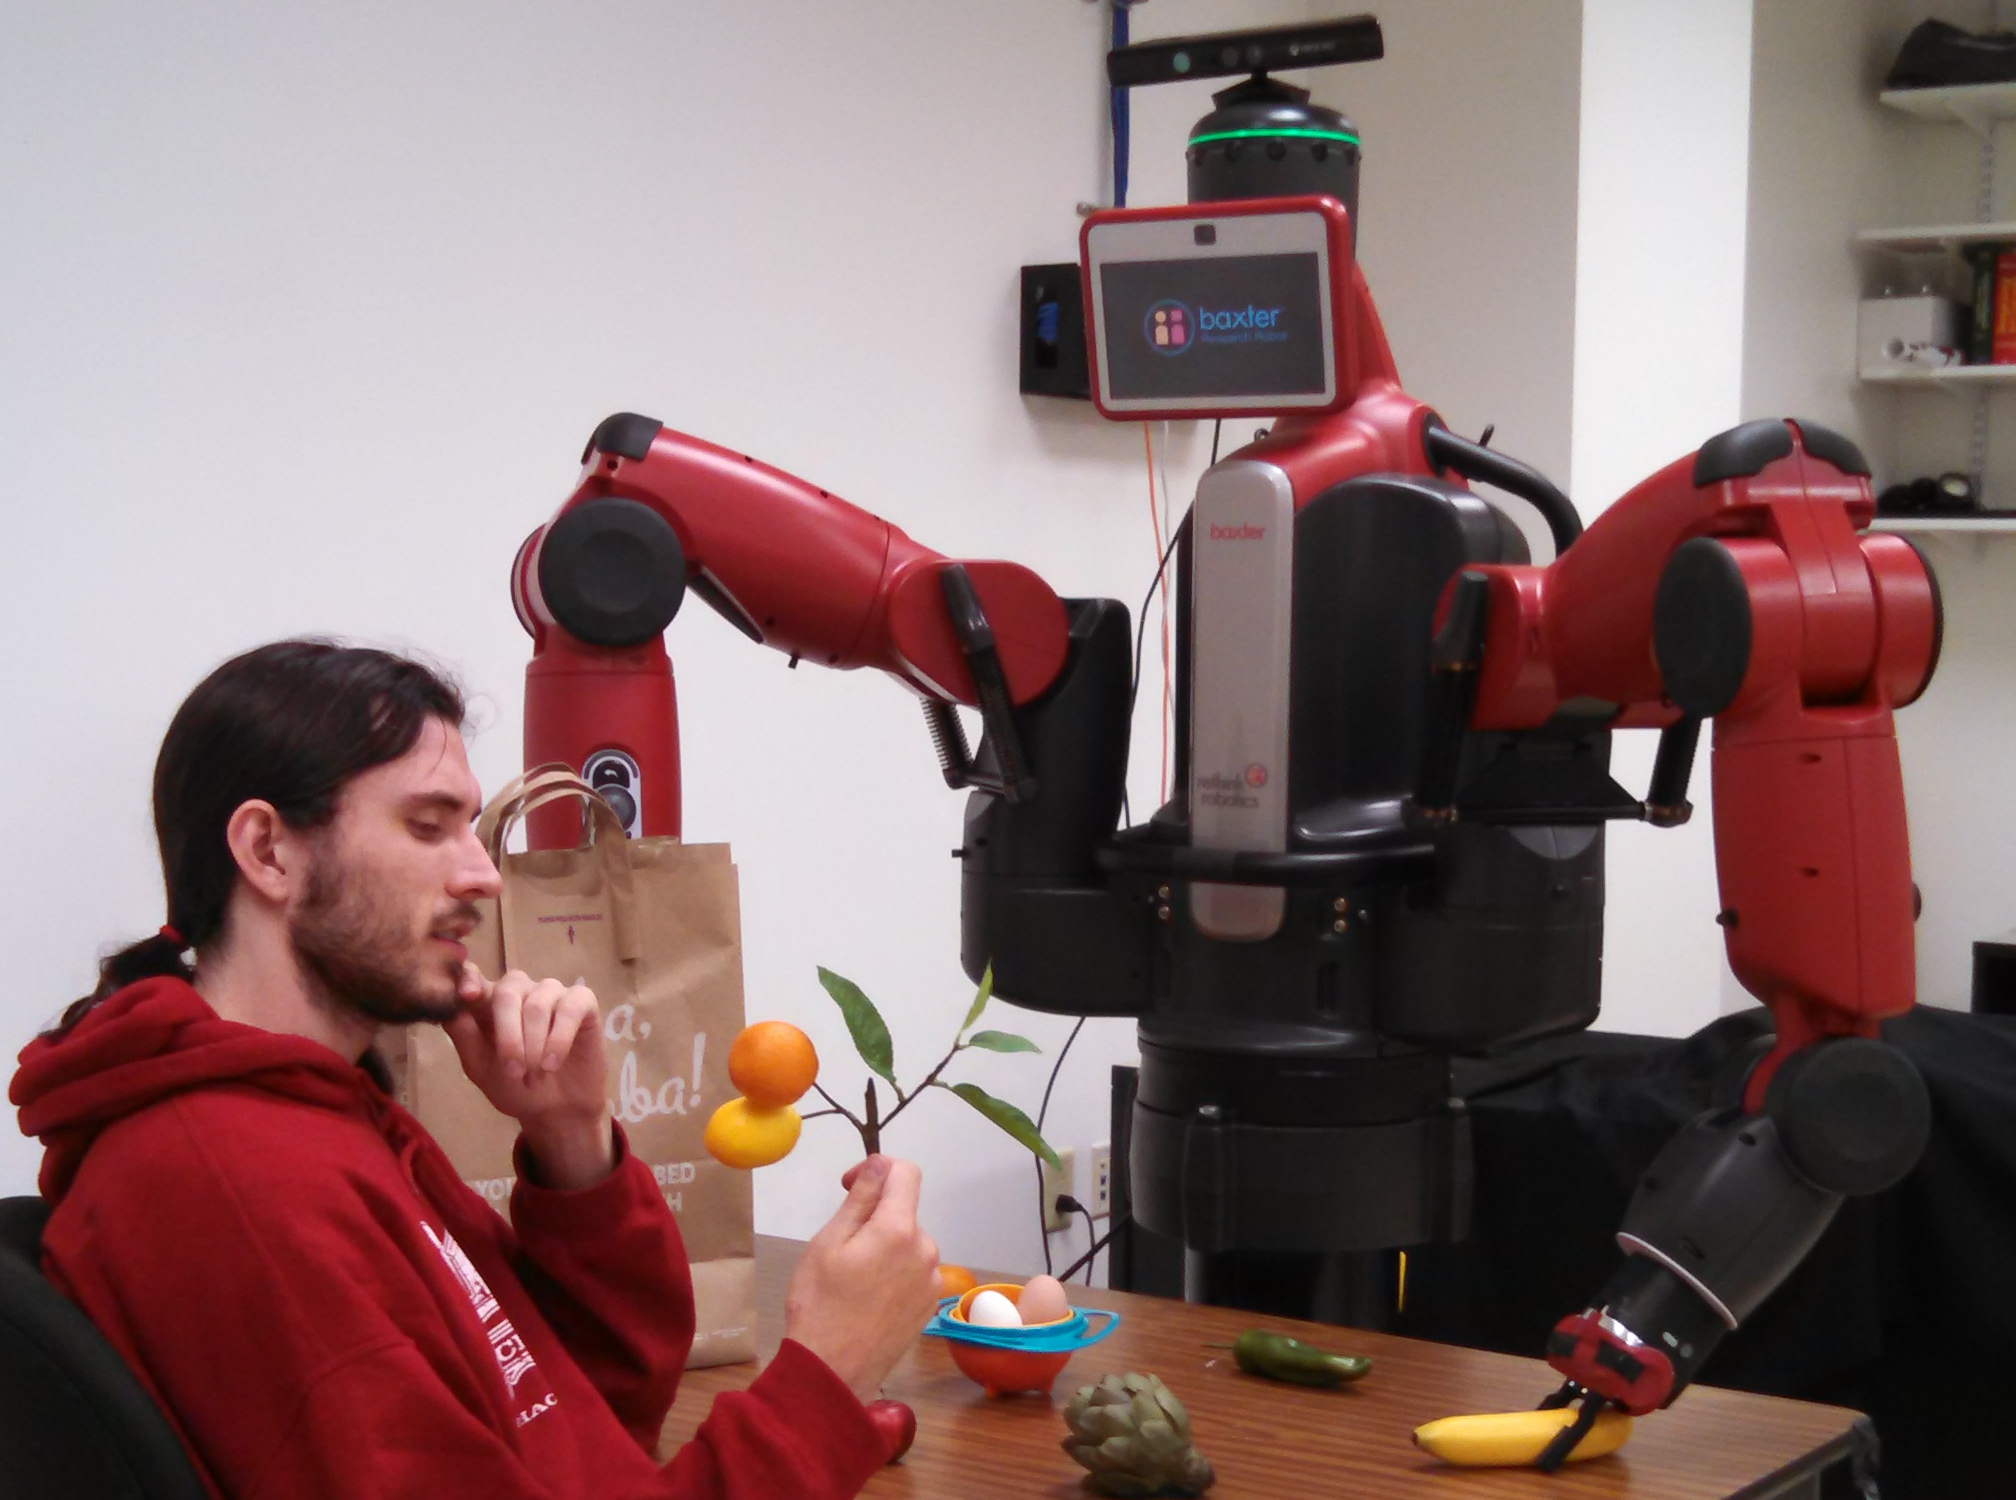
\includegraphics[width=200px, height=150px]{robo2.png} &
      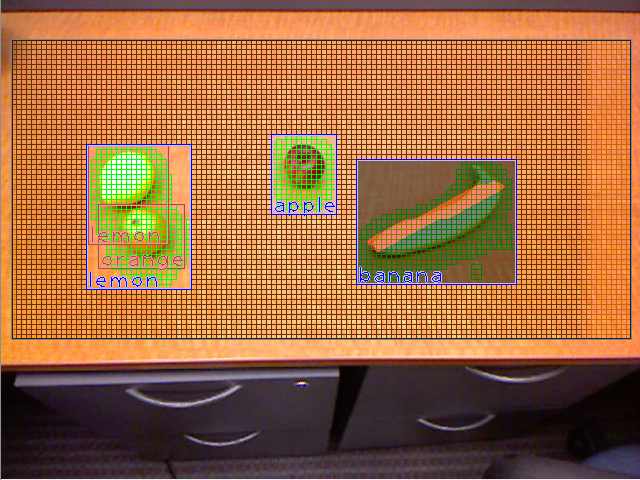
\includegraphics[width=200px, height=150px]{screen2.png} \\
    \end{tabular}
  \end{center}
  \caption{Left: Baxter uses visual servoing to grasp an object. Right: The view through Baxter's wrist camera, 
    showing the location of the target as well as the objective reticle.}
\end{figure*}

\stnote{Cite the visual servoing tutorial paper and talk about the
  connection to grasping rectangles.}

This Grasp Rectangle business fits in nicely with the reticle.

0. Estimate the depth of the table by inspecting non-object locations. This helps decide when to close the gripper.

1. Servo orientation to the '0' orientation, or one of a few sparsely sampled keypoint orientations.
Each viewing orientation (from the wrist) is tied to a grasping orientation.

2. Servo to a 'normal' scale. This is fixed, we don't want multiple scales running around.

3. Now instead of aiming at the center, aim at a proposed target offset from the center.


\subsection{PID Controller}
\jgonote{Maybe a coordinate descent algorithm or wide-scale random noise search.}
Since we use a dual-rate controller, there are two separate sets of coefficients that we must train.
We train the high-rate coefficients with the objective of getting the aim within the ``close'' threshold.
We train the low-rate coefficients with the objective of getting the aim within the 'hit' threshold.
The training for the high and low-rate coefficients is analogous and happens independently, so
without loss of generality we describe the training process for an arbitrary set of coefficients.

\jgonote{I imagine this has been done before so it would be good to find who did this.}
\stnote{Find someone to learn PID coefficients.}
A single set of PID coefficients consists of $K_P$, $K_I$, $K_D$. In the inside loop of EM-like training, we
randomly pick a coefficient $K$ to train, fix the other two coefficients,  and use a local search 
algorithm ~\citep{} to find the optimal value of $K$ conditioned on the fixed values of the other two
parameters. This problem is not necessarily convex and so we run the inside loop of our algorithm
until we have converged to a local minimum.


\section{Simultaneous Localization and Mapping of Tabletop Objects}

We aim to autonomously acquire instance-based models of objects based
on exploration.  To carry out this inference, we follow approaches
based on recursive state estimation~\citep{thrun08} and
SLAM~\citep{durrant06}.  In our approach, the map that the robot is
acquiring is not an occupancy grid or landmark locations, as in
conventional SLAM, but rather knowledge of the appearance and grasp
points of the objects being mapped.  The localization problem is
estimating the pose of these objects at each time step.  We can also
jointly estimate the pose of the robot's end effector, but this pose
is often known with high accuracy in the local coordinate system.  The
graphical model for our approach appears in Figure~\ref{fig:model}.

\begin{figure}
\centering
\includegraphics{model-crop.pdf}
\caption{Graphical model for our proposed approach.\label{fig:model}}
\end{figure}

We define the following variables:
\begin{itemize}
\item $x_t = \left< r_t, o_1 \dots o_k \right>$.  Our state consists of
  the pose of the robot's end effector, $r_t$, along with the pose and
  category of all the objects currently being tracked, $o_1 \dots o_k$.
\item $z_t = \left<r, g, b, d\right>$.  Our observation consists of
  the pixel values and depth generated from a sensor on the robot's
  end effector.  This sensor could be a depth camera from the Kinect;
  in our experiments we use a one-pixel depth camera created from
  Baxter's IR sensor and wrist camera.
\item $u_t = \left\{\left<x, y, z, r, p, y\right>\right.$ Alternately,
  the robot could attempt to grasp the object, leading to a new
  configuration of objects in the workspace.
\item $m$ The map consists of a colored voxel map for each object. 
\end{itemize}

We aim to jointly estimate a distribution over object poses along with
the map, $m$:
\begin{align}
p(x_t, m |  z_0 \dots z_t, u_0 \dots u_t)
\end{align}

We formulate this problem as a Bayes' filter with a time update:
\begin{align}
p&(x_t, m | z_0 \dots z_{t-1}, u_0 \dots u_t) = \notag\\
&\int p(x_t | x_{t-1}, u_t) \times p(x_{t-1}, m | z_{0} \dots z_{t-1}, u_{0} \dots u_{t-1}) dx_{t-1}
\end{align}

and a measurement update: 
\begin{align}
p(&x_t, m | z_0 \dots z_t, u_0 \dots u_t) = \notag\\
&\frac{p(z_t | x_t, m) P(x_t, m | z_0 \dots z_{t-1}, u_0 \dots u_t)}
{p(z_t | z_{0} \dots z_{t-1}, u_0 \dots u_t)}
\end{align}

\subsection{Transition Model}

Our transition model incorporates the effect of the control input on
the robot's end effector as well as on all the objects:
\begin{align}
p(x_t | x_{t-1}, u_t) &= p(r_t, o^1_t \dots o^k_t | r_{t-1}, o^1_{t-1} \dots o^k_{t-1}, u_t) \\
\intertext{We assume that the robot's end effector pose and the object poses are independent:}
                     &= p(r_t | u_t) \times p(o^1_t \dots o^k_t | o^1_{t-1} \dots o^k_{t-1}, u_t)
\intertext{
We also assume that each object is independent of the
others; although in general we would like the robot to predict the
effects of its grasps, in practice other objects can be moved by
mistake.  Therefore our transition model will have high uncertainty
over all objects when the robot moves any object.}
                    &\approx p(r_t | u_t) \times \prod_k p(o^k_t | o^k_{t-1}, r_t)
\end{align}

We endow the robot with two types of control actions.  In the first
type, the robot plans collision free motions with conservative models
of the boundaries of possible objects; these types of transitions move
the robot's end effector but leave all the object poses unchanged.
The second type is when the robot grasps an object.  After an
attempted grasp we assume the pose of all the objects have moved and
need to be reestimated (in case the robot knocked an object during its
attempted grasp)

\subsection{Measurement Model}

Our sensor consists of a depth camera; for simplicity we update one
pixel at a time, although a sensor such as the Kinect would consist of
many updates at once.
\begin{align}
p(z_t | x_t, m) = p(z_t | r_t, o_t^1 \dots o_t^k, m)
%
\intertext{When the object pose and map is known, we can identify the
  one object penetrated by the sensor:}
%
p(z_t | x_t, m) = p(z_t | r_t, o_t^i, m^i)
\end{align}

We assume a sensor model with Gaussian noise on pixel values and depth
values.

\subsection{Inference}

We carry out inference in the model using a Rao-Blackwellized Particle
Filter~\citep{durrant06}.  In particular we partition our state space
according to the product rule:

\begin{align}
p(&x_0 \dots x_t, m | z_0 \dots z_t, u_0 \dots u_t) = \notag\\
& p(m | x_0 \dots x_t, z_0 \dots z_t) \times p(x_0 \dots x_t | z_0 \dots z_t, u_0 \dots u_t)
\end{align}

Thus each particle is represented by the set:
\begin{align}
\left\{ w_t^{(i)}, x_0^{(i)} \dots x_t^{(i)}, p(m | x_0^{(i)} \dots x_t^{(i)}, z_0 \dots z_t)\right\}
\end{align}

In a simplified model, we can compute a maximum likelihood map
analytically from the pose and observation history, rather than
representing a distribution over it.

Our proposal distribution is the motion model, as in Fast Slam
1.0~\citep{montemerlo02}:
\begin{align}
x_t^{(i)} \sim  p(x_t | x_{t-1}^{(i)}, u_t)
\end{align}

That is, when objects do not move, we assume a fixed pose, together
with small random movement to correct initial pose estimation error.


\section{Experimental Setup}
\jgonote{This is where we describe the experiments we performed.}
We are not trying to extend the state-of-the-art on our individual tasks. Rather,
we are providing an interactive framework which will raise the maximum automated vision
available to the average user.

Our system can be evaluated in two important ways. Firstly, how effective is 
the system at the tasks for which it is trained? Secondly, how accessible to users is the system?
For now we evaluate system performance, and leave user studies for future work.

\subsection{Object Detection and Pose Estimation}
For object Detection and pose estimation, we constructed data
sets on which we could evaluate our models. This involved hand
annotating the ground truth for the images in the sets, which is a
costly procedure which we are attempting to eliminate for future tasks.
However, we cannot evaluate our system in a principled fashion without such
a data set.

We demonstrate our method's success in this setting where we pay the cost
to acquire the data so that we can trust our method and that cost need not be 
payed during future applications. 

Probably uses confusion rates as the objective function.

Expert viewpoint collection (uses at least hard negatives)

Super dense sampling

uniform hard negative sampling with stopping criterion

\subsection{Grasp Experiments}
For grasp experiments, we conducted online trials in order to compute success rates.
This uses grasp success rate as an objective function.

Expert annotation of grasps

Uniform grasp sampling

Thompson sampling

\subsection{PID Control Experiments}
For PID experiments, we conducted online trials in order to compute success rates.
We use the time to convergence as the objective function




\section{Evaluation and Discussion}
We could report the performance of the system as a function of user interactions.

We could report the performance of the system as a function of program lifetime.

Our representative set could consist of a block, a spoon,
a bowl, a diaper, and a sippy cup. A \emph{single cut video} showing multiple grasps
of all objects is available here.

\subsection{Object Detection}
We establish a baseline for performance by training the system in a representative domain
specific setting, which tells us how well it can perform on laboratory objects when trained by an 
expert. This represents the best that the system could be expected to perform.

\begin{table}
  \begin{center}
  \caption{Performance of our system on the object detection task.}
  \begin{tabular}{lr}
    \toprule
  Data Collection Method & Success Rate \\ 
  \midrule
  Expert Annotation & 0.0 \\ 
  Dense Sampling & 0.0 \\ 
  Hard Negatives Auto-Stopping & 0.0 \\ 
  \bottomrule
  \end{tabular}
  \end{center}
\end{table}

\subsection{Pose Estimation}

\begin{table}
  \caption{Performance of our system on offline data.}
  \begin{center}
  \begin{tabular}{lr}
\toprule
  Data Set            &  \\ 
\midrule
  Expert Curated      & 0.0 \\ 
  Expert (noisy)      & 0.0 \\ 
  Automatic (curated) & 0.0 \\ 
  Automatic (noisy)   & 0.0\\
\bottomrule
  \end{tabular}

  \end{center}
\end{table}


\subsection{Grasping}

\begin{figure}
  \begin{center}
  \begin{tabular}{lr}
  \toprule
  Grasp Sampling Method & Success Rate \\ 
  \midrule
  Expert Annotation & 0.0 \\ 
  Uniform Sampling & 0.0 \\ 
  Thompson Sampling & 0.0 \\
  \bottomrule
  \end{tabular}
  \caption{Performance of our system on the grasping task.}
  \end{center}
\end{figure}

\subsection{PID Control}

\begin{figure}
  \begin{center}
  \begin{tabular}{lr}
    \toprule
  Parameter Learning Method & Average Convergence Time \\ 
  \midrule
  Expert Annotation & 0.0 \\ 
  Constant Learning Rate & 0.0 \\
  Decaying Learning Rate & 0.0 \\
  Wide Scale Random Noise & 0.0 \\
  \bottomrule
  \end{tabular}
  \caption{Performance of our system on the PID control task.}
  \end{center}
\end{figure}

%\subsection{Laboratory Automatic Training}
%How well does the automatic training system perform when trained in laboratory conditions?

%\subsection{Non-Expert In-The-Wild Training}
%We then go on to compare the performance of the system when trained to various degrees by naive
%and technical non-expert users.
%We repeat the experiments with naive users in two settings. In the first, they train laboratory
%objects. In the second, they provide their own objects.


\section{Related Work}


Summary: 
\begin{itemize}
\item People doing SLAM.  \citet{wang07, gallagher09}, 
\item People doing 3d reconstruction.   \citet{krainin11, banta00}
\item People doing big databases for category recognition.  \citet{kent14a, kent14, lai11a, goldfeder09}
\item Object tracking in vision (typically surveillance).
\item POMDPs for grasping.  \citet{platt11, hsiao10}
\item People doing systems.  \citet{hudson12, ciocarlie14}
\end{itemize}


Crowd-sourced and web robotics have created large databases of objects
and grasps using human supervision on the web~\citep{kent14a, kent14}.
These approaches outperform automatically inferred grasps but still
require humans in the loop.  Our approach enables a robot to acquire a
model fully autonomously, once the object has been placed on the
table.

\citet{zhu14} created a system for detecting objects and estimating
pose from single images of cluttered objects.  They use KinectFusion
to construct 3d object models from depth measurements with a
turn-table rather than automatically acquiring models.

\citet{chang12} created a system for picking out objects from a pile
for sorting and arranging but did not learn object models.  

next-best view planning~\citep{kriegel11}

\citet{banta00} constructs a prototype 3d model from a minimum number
of range images of the object.  It terminates reconstruction when it
reaches a minimum threshold of accuracy.  It uses methods based on the
occluded regions of the reconstructed surfice to decide where to place
the camera and evaluates based on the reconstruction rather than pick
up success.  \citet{krainin11} present an approach for autonomous
object modeling using a depth camera observing the robot's hand as it
moves the object.  This system provides a 3d construction of the
object autonomously.  Our approach uses vision-based features and
evaluates based on grasp success.

\stnote{Need to find the instance-based work that Erik mentioned when
  he said it was a ``solved problem.''}

\citet{velez11} created a mobile robot that explores the environment
and actively plans paths to acquire views of objects such as doors.
However it uses a fixed model of the object being detected rather than
updating its model based on the data it has acquired from the
environment.

Methods for planning in information space \citep{he08, atanasov13,
  prentice09} have been applied to enable mobile robots to plan
trajectories that avoid failures due to inability to accurately
estimate positions.  Our approach is focused instead on
object detection and manipulation, actively acquiring data for use
later in localizing and picking up objects. \stnote{May need to say
  more here depending on what GRATA actually is.}


Early models for pick-and-place rely on has been studied since the
early days of robotics~\citep{brooks83, lozano89}.  These systems
relied on models of object pose and end effector pose being provided to the
algorithm, and simply planned a motion for the arm to grasp.  Modern
approaches use object recognition systems to estimate pose and object
type, then libraries of grasps either annotated or learned from
data~\citep{saxena08, goldfeder09, morales03}.  These approaches
attempt to create systems that can grasp arbitrary objects based on
learned visual features or known 3d configuration.  Collecting these
training sets is an expensive process and is not accessible to the
average user in a non-robotics setting.  If the system does not work
for the user's particular application, there is no easy way for it to
adapt or relearn.  Our approach, instead, enables the robot to
autonomously acquire more information to increase robustness at
detecting and manipulating the specific object that is important to
the user at the current moment.

Visual-servoing based methods~\citep{chaumette06} \stnote{Need a whole
  paragraph about that. }

\stnote{\citet{ciocarlie14} seems highly relevant, could not read from
  the train's wifi.}  Existing work has collected large database of
object models for pose estimation, typically curated by an
expert~\citep{lai11}.  \citet{kasper12} created a semiautomatic system
that fuses 2d and 3d data, but the setup requires a special rig
including a turntable and a pair of cameras.  Our approach requires an
active camera mounted on a robot arm, but no additional equipment, so
that a robot in the home can autonomoulsy acquire new models.

\citet{collect14} describes an approach for lifelong robotic object
discovery, which infers object candidates from the robot's perceptual
data.  This system does not learn grasping models and does not
actively acquire more data to recognize, localize, and grasp the
object with high reliabilitiy.  It could be used as a first-pass to
our system, after which the robot uses an active method to acquire
additional data enablign it to grasp the object.  Approaches that
integrate SLAM and moving object tracking estimate pose of objects
over time but have not been extended to manipulation~\citep{wang07,
  gallagher09, salas-moreno13, selvatici08}.

Our approach is similar to the philosphy adopted by Rethink Robotic's
Baxter robot, and indeed, we use Baxter as our test
platform~\citep{fitzgerald13}.  \stnote{Haven't actually read this
  paper, just making stuff up based on Rod's talks.  Should read the
  paper and confirm.}  Baxter's manufacturing platform is designed to
be easily learned and trained by workers on the factory floor.  The
difference between this system and our approach is we rely on the
robot to autonomously collect the training information it needs to
grasp the object, rather than requiring this training information to
be provided by the user.


Robot systems for cooking~\citep{bollini12, beetz11} or furniture
assembly~\citep{knepper13} use many simplifying assumptions, including
pre-trained object locations or using VICON to solve the perceptual
system.  We envision vision or RGB-D based sensors mounted on the
robot, so that a person can train a robot to recognize and manipulate
objects wherever the robot finds itself.

Approaches to plan grasps under pose uncertainty~\citep{stulp11} or
collect information from tacticle sensors~\citep{hsiao10} using
POMDPs.  \citet{plat11} describe new algorithms for solving POMDPs by
tracking belief state with a high-fidelity particle filter, but using
a lower-fidelity representation of belief for planning, and tracking
the KL divergence.

\citet{hudson12} used active perception to create a grasping system
capable of carrying out a variety of complex tasks.  Using feedback is
critical for good performance, but the model cannot adapt itself to
new objects.



\section{Conclusion}

\stnote{First paragraph:  contributions.  What are the things this paper has done to advance the state of the art?}

\stnote{Next paragraphs: future work, spiraling upward to more and
  more ambitiuos extensions.}

Right now, NODE runs on Baxter. We will port NODE to PR2 and other AH systems.
GRATA could be applied in other domains as well.  What are some examples?


% Intro structure
% First paragraph: What is the problem we are trying to solve? 
% Second paragraph: Why hasn't previous work addressed this problem?
% Third paragraph: What do we propose to do to address this problem?
% Fourth paragraph: What is our high-level technical approach.
% Fifth paragraph: How do we know it works? Why is it cool?
%
% 1. Experimental
%  a. Contribution (Is it new?)
%  b. Execution (Does it work?)
%  c. Demonstration (Is it well understood? were the choices made well?)
% 2. Bureaucratic
%  a. Do we know what we are talking about?
%  b. CYA (Are we polite about it? Are we accidently claiming false novelty?)
%  c. Do they know what we are talking about? (No algebraic geometry plz k thnx.)
% 3. Aesthetic
%  a. Grammar and Spelling
%  b. Vocab and Word Choice
%  c. Prosody (Does it scan? How is the meter?)

\bibliographystyle{plainnat}
\bibliography{main,references}


\end{document}
